We will now see how \gls{pca} can help us to visualise a high-dimensional data set.
This example will be done on the ovarian cancer data set, which is built into Matlab \cite{brunton2019data}.

The data set contains 216 entries of patients and 4000 genes as a feature.
121 of these patients have ovarian cancer, 95 do not.
However, as we will see in the following analysis, the intrinsic dimension of these 4000 features is not high after all.

\begin{figure}[h]
  \centering
  \begin{subfigure}{0.49\textwidth}
      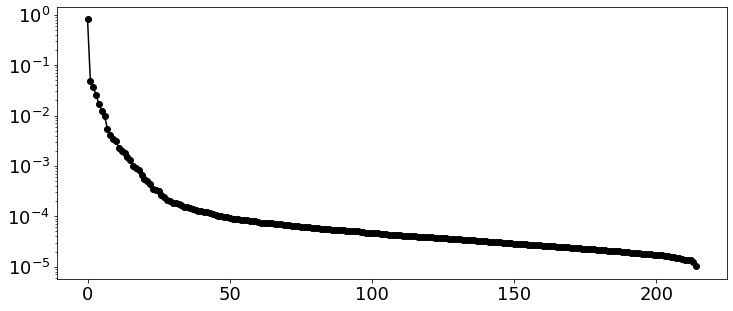
\includegraphics[width=\textwidth]{external_content/media/ovarian_cancer/explained_variance.png}
      \caption{Singular values $\sigma_r$}
      \label{fig:ovarianLog}
  \end{subfigure}
  \hfill
  \begin{subfigure}{0.49\textwidth}
      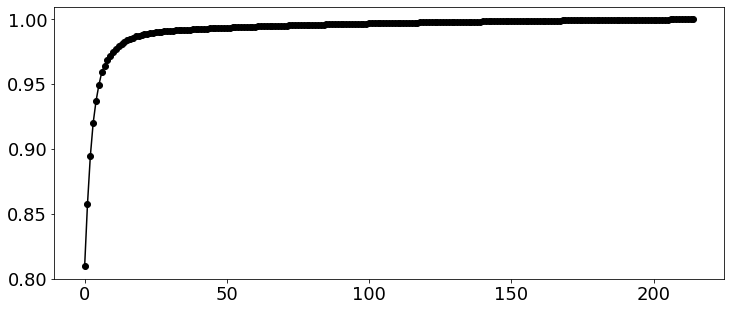
\includegraphics[width=\textwidth]{external_content/media/ovarian_cancer/cumulative_sum.png}
      \caption{Cumulative sum of $\sigma_r$}
      \label{fig:ovarianCumsum}
  \end{subfigure}
  \caption{Singular values of the decomposition of the ovarian cancer data set}
  \label{fig:ovarianSpecs}
\end{figure}


As we can observe in the overview of the singular values in figure \ref{fig:ovarianLog}, the values start converging relatively early at around 30 of 216 singular values.
This is generally desirable as this implies that the values starting at singular value with index 31 carry little information about the data set.
Its importance becomes even more apparent when considering the cumulative sum of the singular values in figure \ref{fig:ovarianCumsum}.


\begin{wrapfigure}[16]{l}{0.6\textwidth}
    \centering
    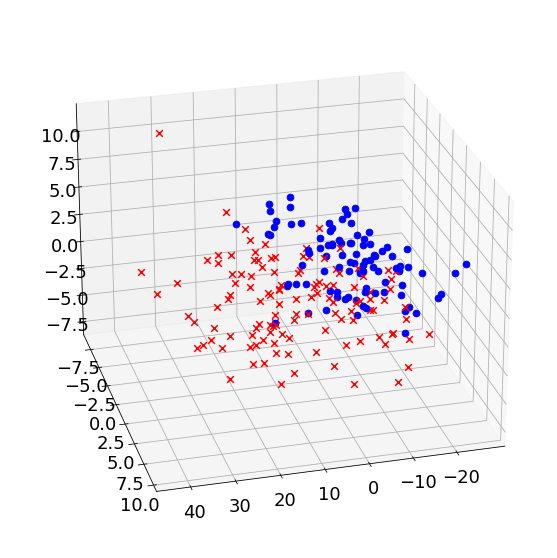
\includegraphics[width=0.94\linewidth]{external_content/media/ovarian_cancer/visualisation.png}
    \captionsetup{justification=centering}
    \caption{Visualisation}
    \label{fig:visualisation}
\end{wrapfigure}

\noindent
We can hereby identify that the first 3 principal components of the data set carry a total of almost 90\% of the total information.
This is while utilising a mere 0,075\% of the originating information.

And since we are now considering 3 dimensions, the data can be elegantly visualised in a 3-dimensional plot as seen on the left side in figure \ref{fig:visualisation}.
As we can see, the patients with and without ovarian cancer concentrate within their respective cluster.



% \item ovarian cancer data set
% \item about 200 patients
% \item 4000 features
% \item all the same unit
% \item ideal for the problem
% \item 3 dimensions preserve 90\% of the information
% \item Grouping is now visible in a 3D plot
